\section{Evaluation}\label{sec:eval}



In this section, we transition from theoretical design to empirical validation. Our evaluation is designed to measure the extent to which our hybrid agentic framework bridges the gap between \emph{descriptive reality} (ambiguous human inputs) and \emph{normative optimality} (mathematical best practices). Specifically, we aim to quantify the efficiency loss incurred when relying on the approximate reasoning of general-purpose LLMs rather than explicit stochastic optimization. By carefully isolating sources of error through controlled baselines, we seek to understand not only \emph{if} the system works, but also \emph{why} standard foundation models fail in this domain.


We address three primary research questions:

\begin{enumerate} 
\item \emph{Efficacy:} Does our hybrid architecture, by decoupling semantic understanding from logical optimization, outperform advanced commercial models (e.g., \emph{GPT-4o}) on complex stochastic inventory control tasks?

\item \emph{Structural Robustness:} Are the performance gains stable across varying degrees of environmental complexity? Under what conditions does our agentic framework achieve the largest marginal improvements?

\item \emph{Limits of Prompt-Based Reasoning:} Can the reasoning failures of general-purpose LLMs be remedied simply by providing perfect, ground-truth problem specifications? Or does stochastic optimization mark a fundamental \emph{computational boundary} that probabilistic language models cannot reliably cross without additional algorithmic and architectural support?

\end{enumerate}



\subsection{Evaluation Pipeline: An \textit{In Silico} Laboratory}


To empirically validate the Hybrid Agentic Framework proposed in \Cref{sec:framework}, we construct a controlled \textit{in silico} experiment using the Human Imitator developed in \Cref{sec:imitator}. This experimental design allows us to stress-test the system under realistic conversational friction, including ambiguity, inconsistency, and non-technical phrasing, while avoiding the logistical and financial constraints of large-scale human-subject trials.

Notably, this evaluation protocol generalizes beyond inventory management. By employing a high-fidelity synthetic agent to simulate the human-in-the-loop, our approach provides a scalable and reproducible testbed for evaluating a wide range of interactive LLM tasks where human variability and latent business knowledge are critical factors.


\subsubsection{Experimental Protocol.}\label{sec:protocol}
The evaluation protocol for each trial follows a three-stage lifecycle, as illustrated in \Cref{fig:evaluation}:

\begin{figure}[!t]
    \centering
    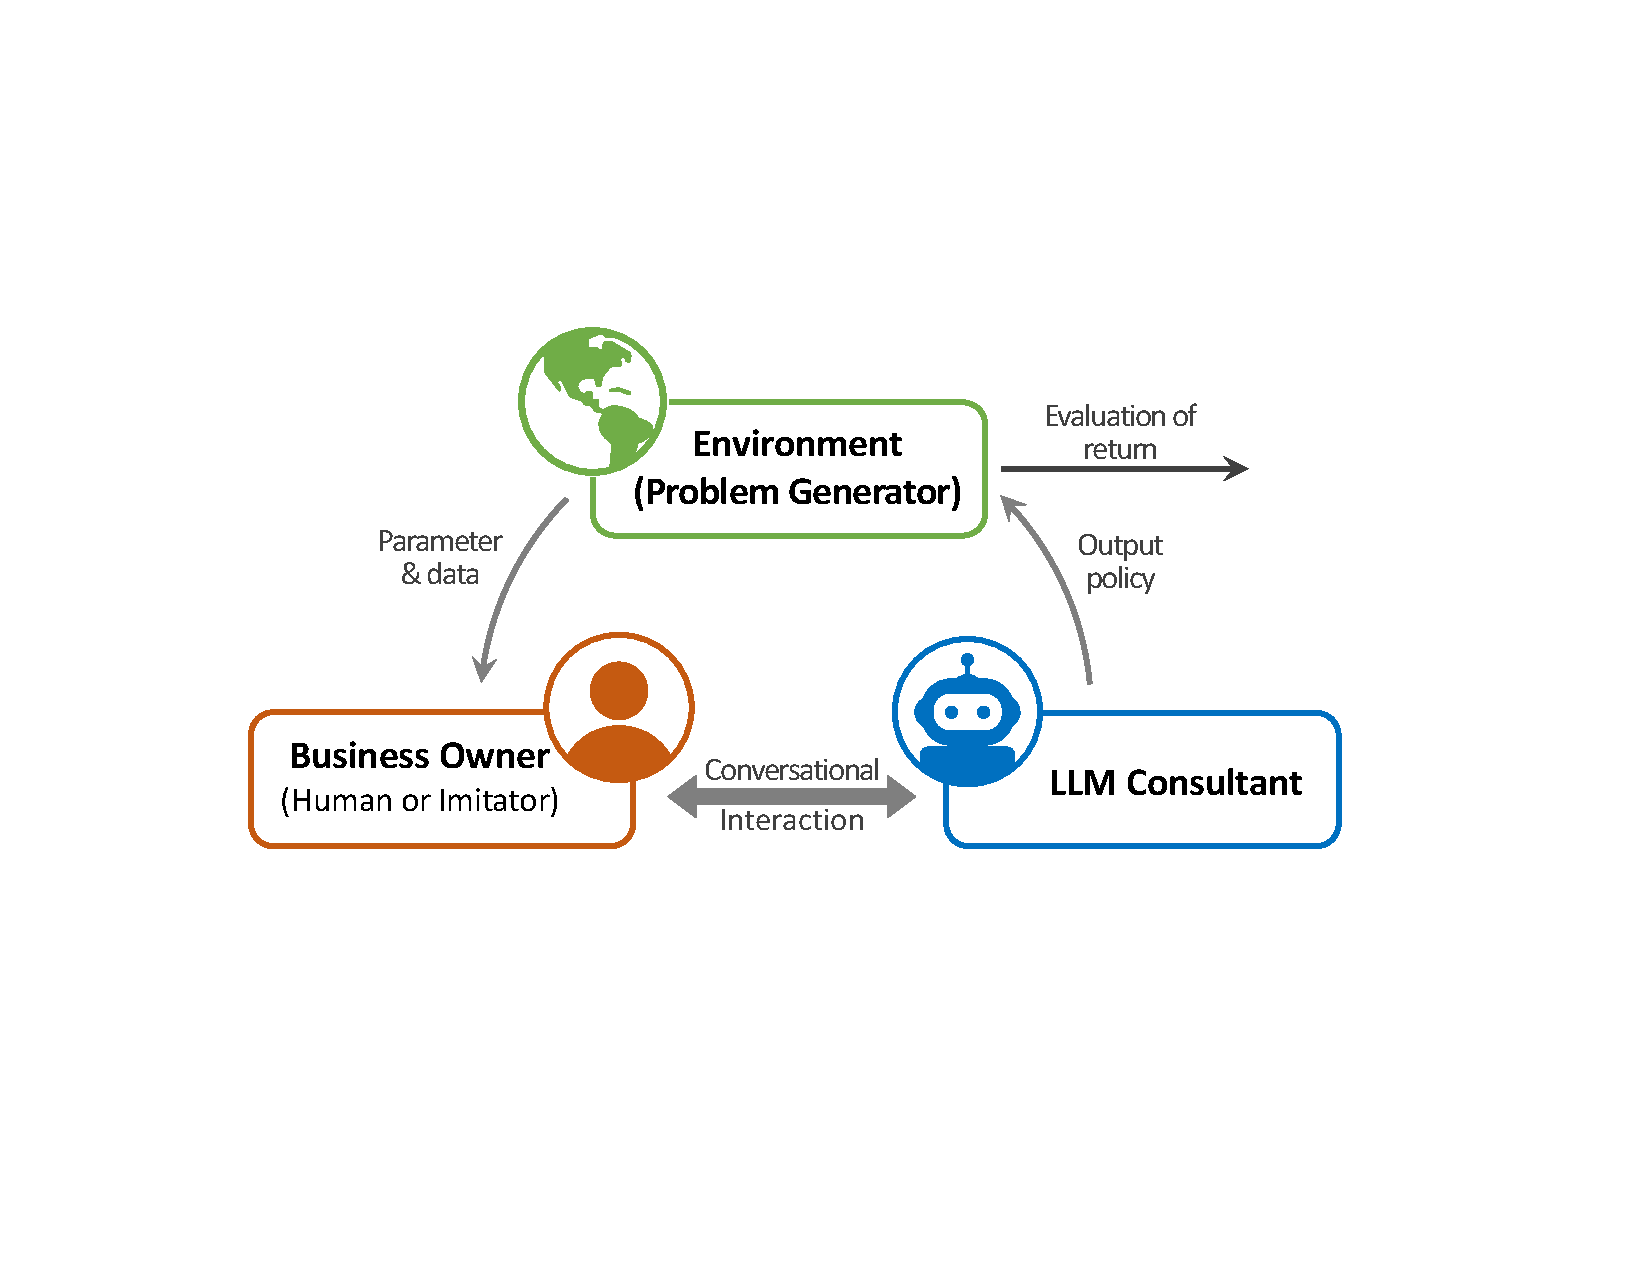
\includegraphics[width=0.75\linewidth]{fig/evaluation_new.pdf} 
    \caption{\textbf{Evaluation Protocol.} The workflow moves from latent ground-truth generation \\ to conversational extraction, culminating in objective policy assessment.}
    \label{fig:evaluation}
\end{figure}

\begin{description}
    \item[1. Initialization (Ground Truth Generation):]
    The process begins with a {Problem Generator Agent}, implemented using \emph{GPT-4o}, which procedurally generates unique inventory management instances. Each instance comprises a high-level semantic context (e.g., ``Managing imported ingredient inventory for a premium restaurant'') and a precise set of \textit{ground-truth parameters} \footnote{When generating parameters, we follow standard parameterizations in the inventory management literature. For example, the inventory holding cost is set to 30\% of the item cost; the standard deviation of demand is approximately one-third of the mean; and the \emph{critical ratio}, defined as \texttt{penalty\_cost} / (\texttt{penalty\_cost} + \texttt{holding\_cost}), typically lies between 0.8 and 0.9.} (\Cref{tab:param-definitions}). These parameters constitute the ``latent reality'' of the business, representing details that a manager might intuitively grasp or access via records, yet struggles to articulate formally due to partial awareness or bounded rationality. Crucially, these ground-truth values provide the definitive benchmark against which all policies subsequently generated by the systems are evaluated.



    \begin{table}[!ht]
    \centering
    \renewcommand{\arraystretch}{1.2}
    \begin{tabular}{
        >{\raggedright\arraybackslash}p{0.26\textwidth}
        >{\raggedright\arraybackslash}p{0.705\textwidth}
    }
        \toprule
        \textbf{Parameter} & \textbf{Description} \\
        \midrule
        \texttt{time\_horizon} &
        The planning period for inventory decisions (default unit: days). \\

        \texttt{demand\_type} &
        The nature of customer demand, categorized as either \textit{deterministic} or \textit{random}. \\

        \texttt{demand\_distribution} &
        If deterministic, a constant value; if random, a statistical distribution (e.g., Normal($\mu=30, \sigma=10$)). \\
        & {\footnotesize (\emph{While our experiments primarily utilize Normal or Poisson distributions for simplicity, the framework supports a ``Custom'' setting that allows the system to infer distributions directly from user-uploaded historical data.})} \\

        \texttt{perishability} &
        A boolean value indicating if the items expire. \\

        \texttt{state\_transition\_model} &
        The outcome of a stockout, modeled as either a \textit{lost sale} or a \textit{backlog}. \\

        \texttt{holding\_cost} &
        The cost to store one unit of inventory for a specific time period. \\

        \texttt{penalty\_cost} &
        The cost incurred for each unit of unmet demand. \\

        \texttt{setup\_cost} &
        The fixed cost associated with placing an order. \\

        \texttt{lead\_time} &
        The time delay between placing an order and receiving it. \\

        \texttt{max\_inventory} &
        The maximum allowable inventory level. \\

        \texttt{max\_order} &
        The maximum quantity that can be ordered at one time. \\

        \texttt{risk\_tolerance} &
        An integer $\lambda$ in $\{ -10,-9, -8, \ldots, 9, 10\}$, where a lower value indicates higher risk aversion. \\
        \bottomrule
    \end{tabular}
    \caption{\textbf{Inventory Environment Parameters.} These variables define \\ the ground truth against which all policies are evaluated.}
    \label{tab:param-definitions}
\end{table}

    
    \item[2. Interaction:]
    We initialize the Human Imitator with the latent reality provided by the generator. It then engages a target system (selected from the treatment groups in \Cref{sec:benchmarks}) in a natural language dialogue. Crucially, the Imitator simulates the opacity of real-world consulting: rather than transmitting structured parameters directly, it describes the business situation conversationally, revealing information only through narrative descriptions and responses to follow-up inquiries, while maintaining realistic levels of ambiguity.
    
    \item[3. Assessment (Policy Evaluation):]
    Once the system proposes a policy, we evaluate its performance against the original \textit{ground-truth} parameters (distinct from the parameters the system may have inferred). We estimate the expected cost and standard deviation via Monte Carlo simulation.
    To accommodate different output formats, we employ a unified evaluation protocol: 
    \begin{itemize}[label=-]
        \item \emph{Automated Evaluation:} For standard mathematical policies (specifically Deep RL, $(s, S)$, or $(R, Q)$\footnote{The $(R, Q)$ policy is an inventory control strategy where a fixed quantity $Q$ is ordered whenever the inventory position drops to or below the reorder point $R$.}), our system automatically parses the parameters and executes the simulation.
        \item \emph{Manual Translation:} For policies proposed by baseline methods that do not fit these categories, we manually translate the described logic into executable code to ensure they are evaluated fairly.
    \end{itemize}
    Finally, we compute the optimality gap between the proposed policy and the theoretical benchmark.
\end{description}

This procedure is repeated across multiple trials to generate diverse inventory problem instances. Given that optimal costs vary significantly in magnitude across different scenarios, we report the relative cost difference between algorithms.

\subsubsection{Experimental Conditions (Baselines).}\label{sec:benchmarks}
To isolate the sources of performance gain, we compare our proposed framework (in \Cref{sec:framework}) against two distinct \emph{GPT-4o} baselines. This comparative design allows us to decompose decision error into \textit{epistemic error} (translation failure) and \textit{computational error} (optimization failure).
\Cref{fig:treatment} provides a schematic overview of this experimental architecture, mapping the information flow from the latent ground truth (Environment) to the final mathematical policy (output) for each treatment.







\begin{figure}[!t]
    \centering
    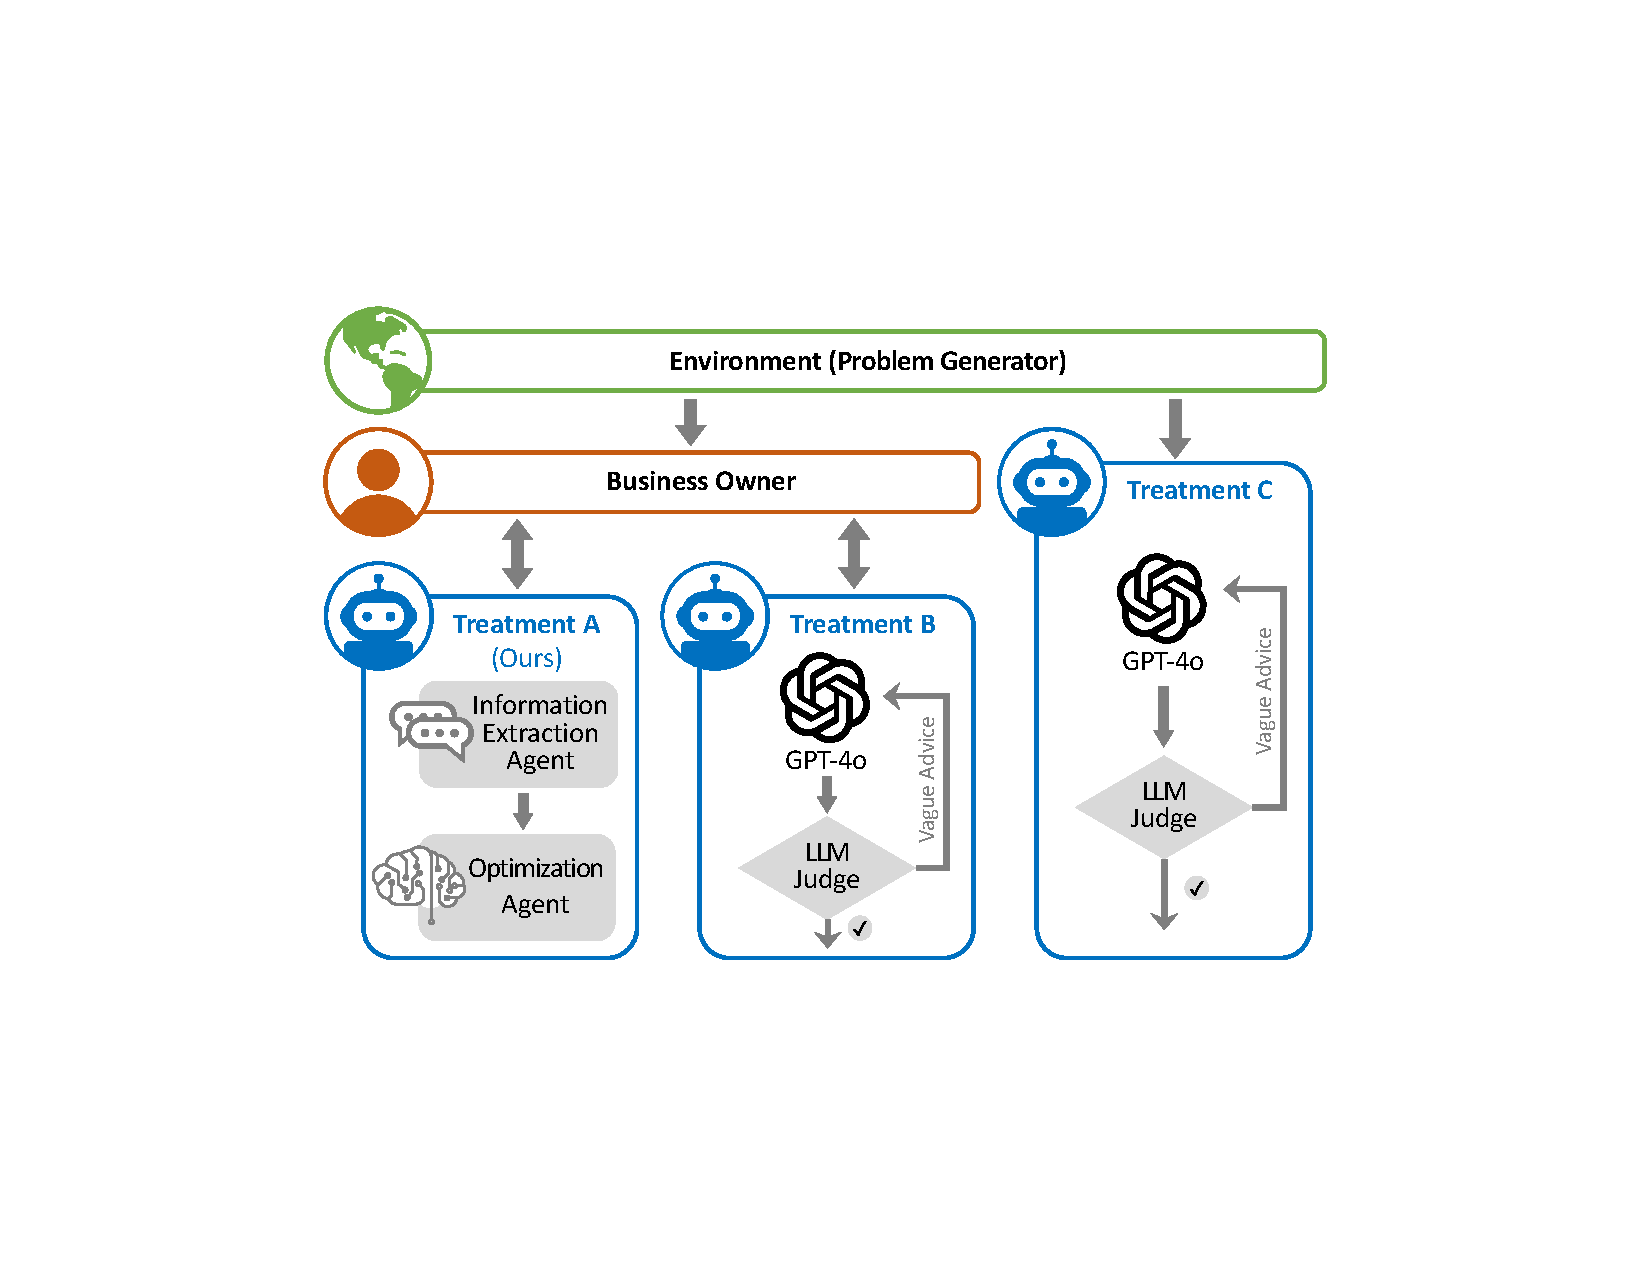
\includegraphics[width=0.7\linewidth]{fig/treatment.pdf} 
    \caption{\textbf{Overview of the comparative experimental framework.}}
    \label{fig:treatment}
\end{figure}



\begin{description}
    \item[\textbf{Treatment A:} Interactive Hybrid Agent (Ours).] 
    This is the full proposed architecture in \Cref{sec:framework}. The system must navigate the conversation with the Human Imitator to extract parameters into a structured format (\Cref{tab:initial_params}) and then employ its internal Optimization Agent to compute a normative policy, using either a grid search for optimal $(s, S)$ thresholds or Deep Reinforcement Learning to handle complex, high-dimensional state spaces.

    

    \item[\textbf{Treatment B:} \textit{GPT-4o} (Interactive).] This baseline represents the standard ``End-to-End'' LLM approach. To ensure a rigorous and fair comparison, the Human Imitator initiates the conversation with the identical starting context used for Treatment A, the Hybrid Agentic System. Operating without access to external algorithmic solvers, the model must simultaneously navigate the dialogue context, infer the underlying operational parameters, and derive a policy based solely on its internal probabilistic weights. This treatment specifically tests the capacity of general-purpose models to overcome epistemic barriers and perform complex stochastic reasoning within a purely natural language interface.


    \item[\textbf{Treatment C:} \textit{GPT-4o} (Parameter Input).]
    This non-interactive baseline assesses the model's intrinsic inventory optimization capabilities under conditions of \textit{perfect information}. To bypass the ambiguity associated with conversational extraction, we directly feed the \textit{ground-truth parameter file}, a structured representation of the latent reality, to \emph{GPT-4o}, rather than relying on narrative extraction. The model is then explicitly prompted to derive an optimal policy. This counterfactual setup isolates computational reasoning from linguistic interpretation, allowing us to investigate whether the performance bottleneck in interactive settings stems from dialogue opacity or the model's fundamental algorithmic limitations.
\end{description}
\vspace{.5em}


\paragraph{Control Measures and Prompting.}
To ensure fairness and consistency, both \emph{GPT-4o} baselines (Treatments B \& C) are subject to strict output controls. Specifically, they are prompted with the following instruction to ensure the generation of \textit{evaluable policies} that are easily translatable into mathematical formulas, rather than vague qualitative advice:
\begin{tcolorbox}
    \scriptsize   
The final recommendation must have clear numbers, specify actions for all possible scenarios, and be easily translatable into a mathematical formula.

For example, ``When inventory falls below 20 units, order 80 units'' is a strategy.

``I recommend an (s, S) policy: when the sum of on-hand and on-order inventory drops below 35 units, order up to a total of 150 units'' is also a clear strategy.

``We should consider optimizing inventory'' or ``You need a better plan'' are not strategies.
\end{tcolorbox}
Without this instruction, \emph{GPT-4o} often generates underspecified recommendations—such as ``you need to order more when inventory is below 5 units''—which cannot be explicitly deployed or analyzed in simulation.

To operationalize these constraints, we further employ an auxiliary \textit{LLM Judge} (built on \mbox{\emph{GPT-4o}}). This judge monitors the response stream and acts as a termination mechanism: it validates whether the output contains a well-defined numerical policy and, upon confirmation, halts the generation to archive both the conversation log and the extracted policy for simulation.



%%%%%%%%%%%%%%%%%%%%%%%%%%%%%%%%
